% figures/ch08/fig03-pde-pte-bits.tex — auto-extracted from chapter source
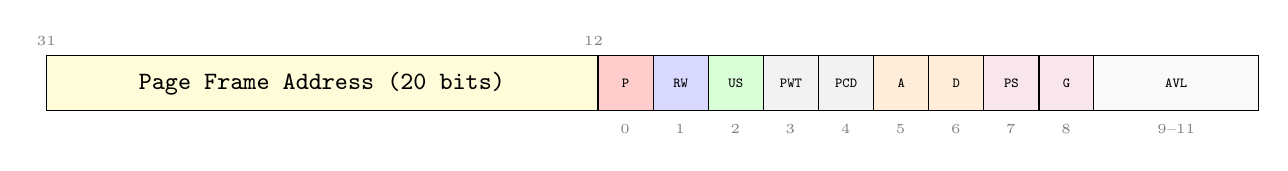
\begin{tikzpicture}[
  bitcell/.style={draw, minimum width=0.7cm, minimum height=0.7cm, font=\ttfamily\tiny, anchor=west},
  bitlabel/.style={font=\tiny, text=gray},
]
  % 高 20 位 — 页帧地址
  \node[draw, minimum width=7cm, minimum height=0.7cm, fill=yellow!15, font=\small\ttfamily]
    (frame) at (0, 0) {Page Frame Address (20 bits)};
  \node[bitlabel, above] at (-3.5, 0.35) {31};
  \node[bitlabel, above] at (3.45, 0.35) {12};

  % 低 12 位 — flags
  \foreach \i/\txt/\col in {
    0/P/red!20,
    1/R\/W/blue!15,
    2/U\/S/green!15,
    3/PWT/gray!10,
    4/PCD/gray!10,
    5/A/orange!15,
    6/D/orange!15,
    7/PS/purple!10,
    8/G/purple!10
  } {
    \node[bitcell, fill=\col] (b\i) at (3.5+\i*0.7, 0) {\txt};
  }
  % AVL bits 9-11
  \node[draw, minimum width=2.1cm, minimum height=0.7cm, fill=gray!5, font=\ttfamily\tiny]
    (avl) at (9.8+1.05, 0) {AVL};

  % bit 标注
  \foreach \i/\b in {0/0, 1/1, 2/2, 3/3, 4/4, 5/5, 6/6, 7/7, 8/8} {
    \node[bitlabel, below] at (3.5+\i*0.7+0.35, -0.4) {\b};
  }
  \node[bitlabel, below] at (10.85, -0.4) {9--11};
\end{tikzpicture}
